\chapter{User Interface Specification}
\label{uispec}
% This section contains mockups, descriptions,
% and explanations, lots of graphics
\section{Preliminary Design}

The user interface (UI) for Paramount Invesments Leagues will act as a command center
for users to interact with their portfolio, leagues they are a part of, and conduct
research on potential orders. More specifically, the command center will act as the
primary; but not the only; view for users to interact with the system.  The command
center will provide a snapshot of the users current portfolio and its value, their
global rank, a dash to perform market orders, a news feed, and a graphing dash in order
to quick analysis of stock performance.  The UI will persist a users global rank across
all views as well as a ticker of current trades being placed through the Paramount
Investment League.\\

The UI should be lightweight so as not to burden our more restrictive target platforms
of mobile and tablet.  The colorscheme will be chosen to be easy on the viewer, though
this is subjective, the colorscheme will be a basic pallet of grey/black/white/blue,
tending toward pastel and web supported colors.\\

The UI will be built on top of Twitter's open source Bootstrap CSS\cite{wiki:boot}
framework to help
facilitate deleriving content to the three target platforms, desktop, mobile, and tablet.
Bootstrap provides a mobile first design philosophy, but can be customized to target
specific platforms.\\

\subsection{Landing Page and Login}

Paramount Invesment League is designed around allowing users to easily begin using the
service, also know as "zero effort" resgistration. In order to accomplish this, the
system does not require the user to register a new user name/account with our system,
but instead piggybacks on OpenID\cite{wiki:open} and OAuth\cite{wiki:oauth} allowing users to
use their Google,
Facebook, Twitter, and other OpenID/OAuth accounts to login. You'll also notice that
upon initial visit, the header is empty providing no navigation, this may be relaxed in
the future to allow the user to explore some of the features of the website that don't
require user authentication such as stock research. (\em See figure 3.1 \em)\\

\begin{figure}
\centering
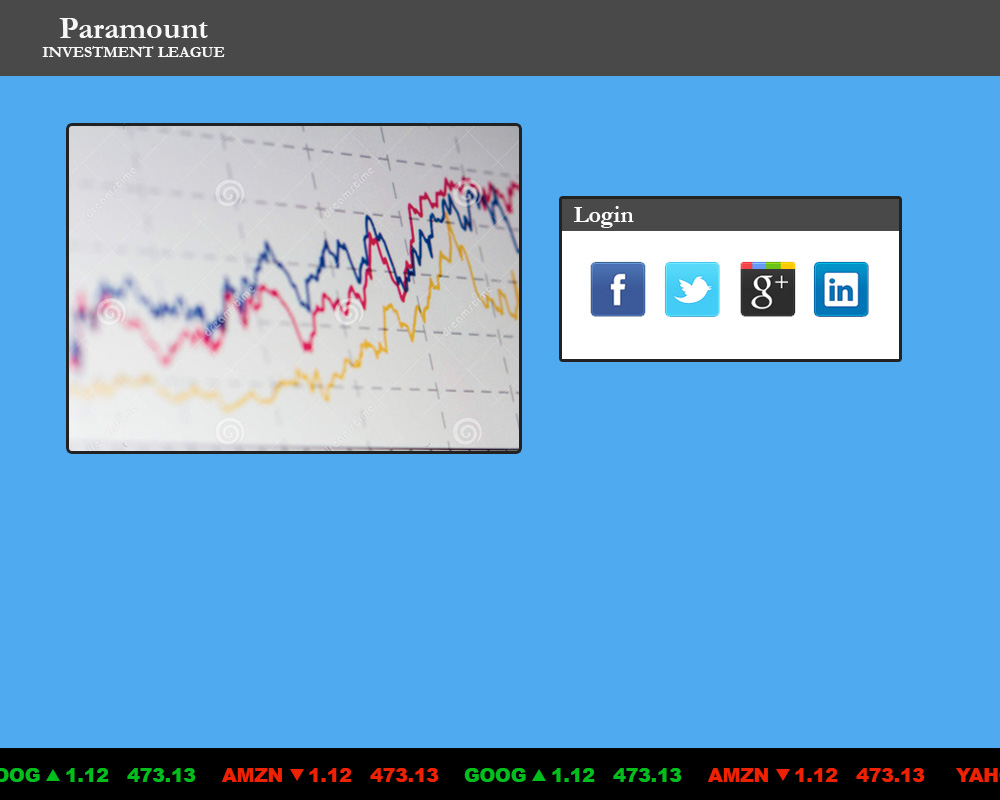
\includegraphics[width=5.5in]{./img/mock/login.jpg}
\caption{First iteration of Landing/Login page.}
\end{figure}

\subsection{Global Header}

The header (\em see Figure 3.2 \em)across the website will remain persistant across the
website once the user is logged into the system.  Navigation is done between essentially
4 views in the following order, My Portfolio, Stock, League, Leaderboard,.  These names
are placeholders and will most likely be My Portfolio, My Leauges, Leaderboards,
Analyze Assets. The 'My Leagues' and 'Leaderboards' will be turned into drop downs as
users expand into leagues to allow quick navigation.\\

The website name will also navigate to My Portfolio. The username will be replaced by the
users actual username, and below it will be the users global rank.  The rank will be
highlighted in red or green depending on whether they have improved their position on the
day, or it has declined.  It will also indicate how many spots they have moved.\\

\begin{figure}
\centering
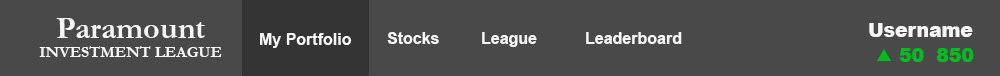
\includegraphics[width=5.5in]{./img/mock/topbar.jpg} %change with header
\caption{Preliminary design for a global header. This users is up 50 spots for the day.}
\end{figure}

\subsection{Global Ticker}

One interesting feature of Paramount Investment Leagues will be its active ticker at the
bottom of the website.  This ticker will be seen in all views, including the Landing Page
once there is enough volume to keep the ticker full.  The ticker serves two goals, one for
new users, and one for existing users.  The first goal is to entice new users to
participate by demonstrating that the app is being widely used. The second goal is to give
a snapshot to existing users of assets that are "on the move" so that they can attempt to
remain competetive. The ticker can be seen at the bottom of all the figures.\\

\subsection{My Portfolio}

The 'My Portfolio' (\em see Figure 3.3 \em) view of the  website will act as the command
center for a user wanting to get news about companies/assets in their portfolio, perform
an order, or conduct quick graphical anaylsis of assets in their portfolio and compare
them to any other asset available for trade through the platform.\\

More importantly, it provides a snapshot of the users portfolio including a scrollable list
of all the assets inside the portfolio and a summary of said assets.  In the future, assets
will be 'clickable' and will take the user to a summary page of that asset, but that is not
planned for the initial 2 iterations.\\

\begin{figure}
\centering
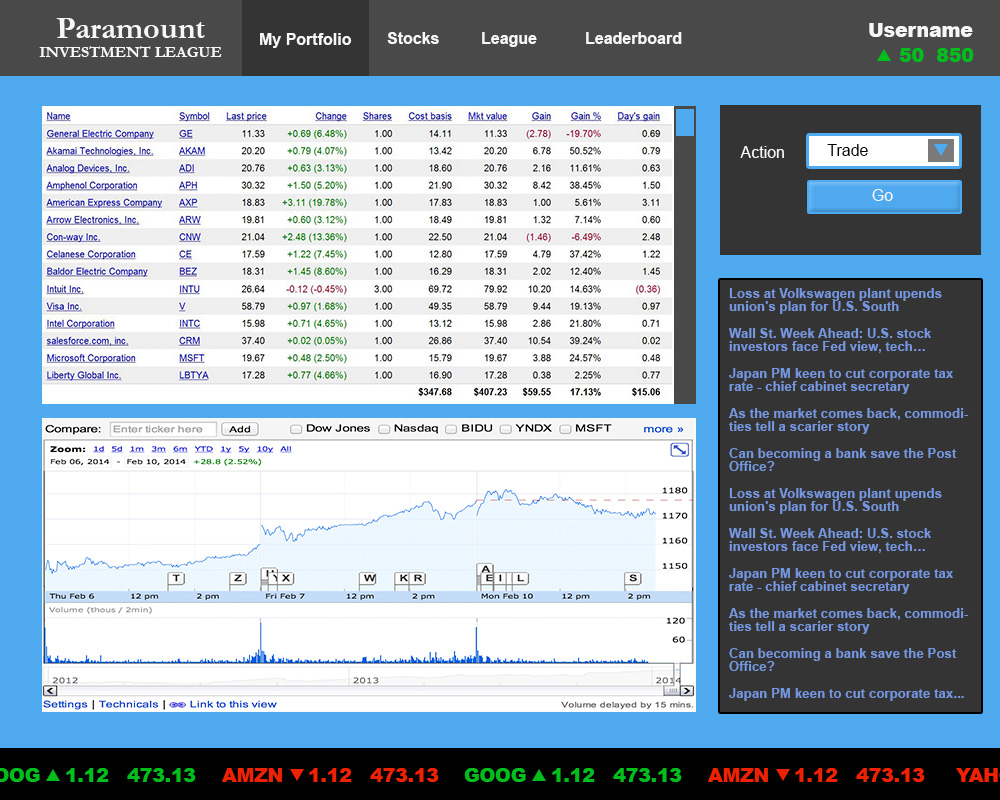
\includegraphics[width=5.5in]{./img/mock/portfolio.jpg}
\caption{The preliminary design of the 'My Portfolio' view.}
\end{figure}

\subsection{Leagues}

The 'League' (\em see Figure 3.4 \em) view will present a user that isn't a part of a league
the ability to create a new league of join an existing league.  Not shown in
\em Figure 3.4 \em is the view that a user who is a part of a league.  This view will still
persist the join/create dialogues, but will also present a list of all the leagues that user
is a part of, their rank within said league, and their movement within said league.\\

\begin{figure}
\centering
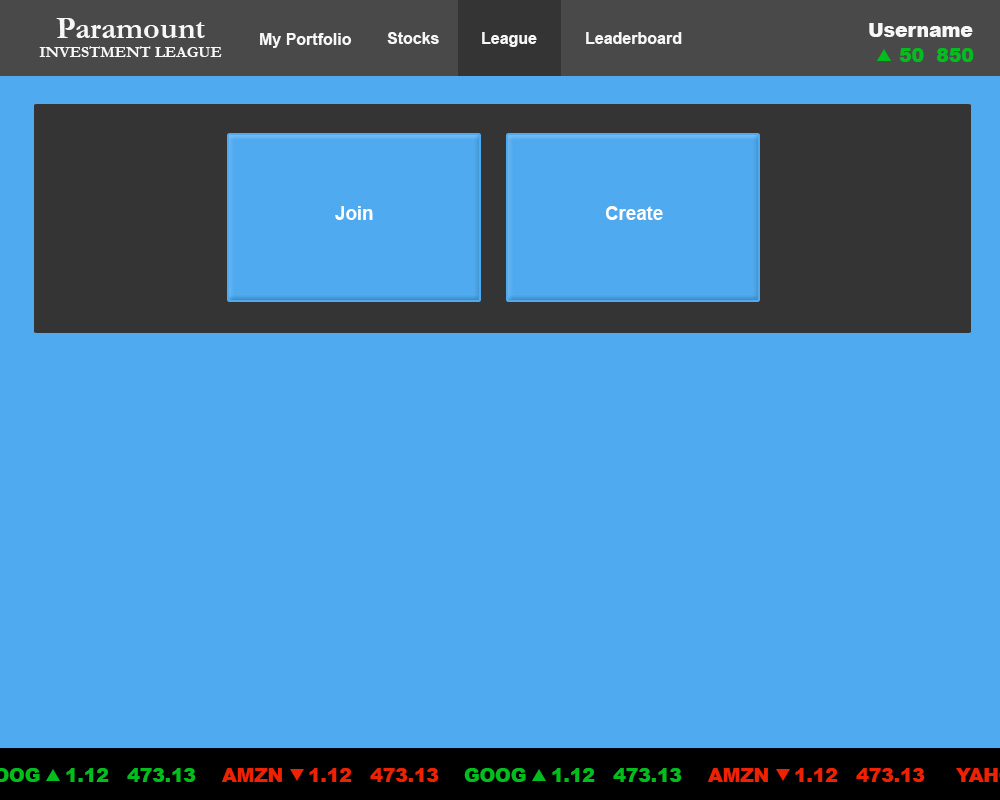
\includegraphics[width=5.5in]{./img/mock/league.jpg}
\caption{This is the league creation/join view. This would be the view presented to a user
that is a part of no league yet.}
\end{figure}


\subsection{Leaderboards}

The 'Leaderboards' (\em see Figure 3.5 \em) view will present the user with a partial view
of the full leaderboard for a given league, or for every user.  It will show their rank,
their movement, the value of their portfolio as well as the same stats for all other users
around them.  The view will be scrollable if there are more records then can be displayed,
and will center the user in the middle of the view unless they are at the top or bottom
of the board.\\

\begin{figure}
\centering
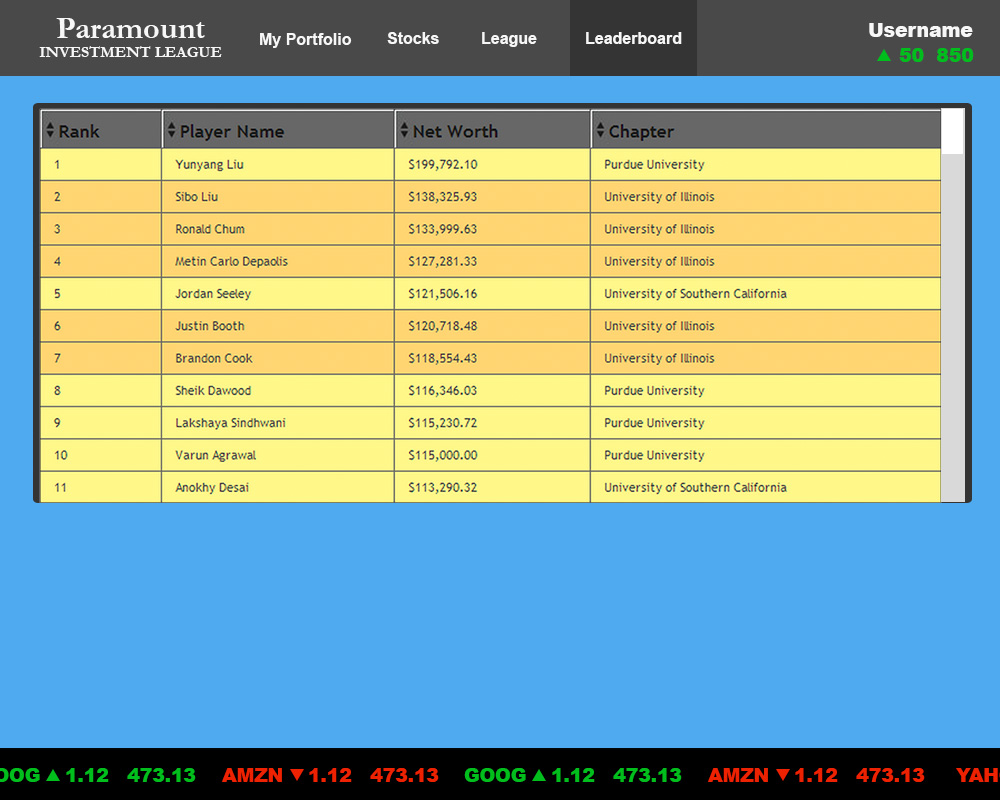
\includegraphics[width=5.5in]{./img/mock/leaderboard.jpg}
\caption{Here is the leaderboard view which will be the same for both leagues and global
leaderboards. This view represents a global leader board.  The colorscheme of this view
here is incomplete and will fall inline with the remainder of the site.}
\end{figure}

\subsection{Asset Analysis}
The 'Stocks' view (\em see Figure 3.5 \em) will be renamed to more align its function
with its name, which is to analyze assets. It will a more in depth way of anaylzing an
asset versus what is available in the 'My Portfolio' view.  There will be a news feed
at the bottom of assets that you are searching for. There will also be a more formal
analysis of asset data presented including P/E ratio, 52 week range, Volume, EPS, etc.
This isn't shown in the figure, but will one-half to two-thirds of the space that
has been set aside for the news feed.\\

This is also one of the views and functionalities that has been identified to not require
the user to be logged in.  While it will not be availble to non-users in the intial product,
it can be made available in future releases.\\

\begin{figure}
\centering
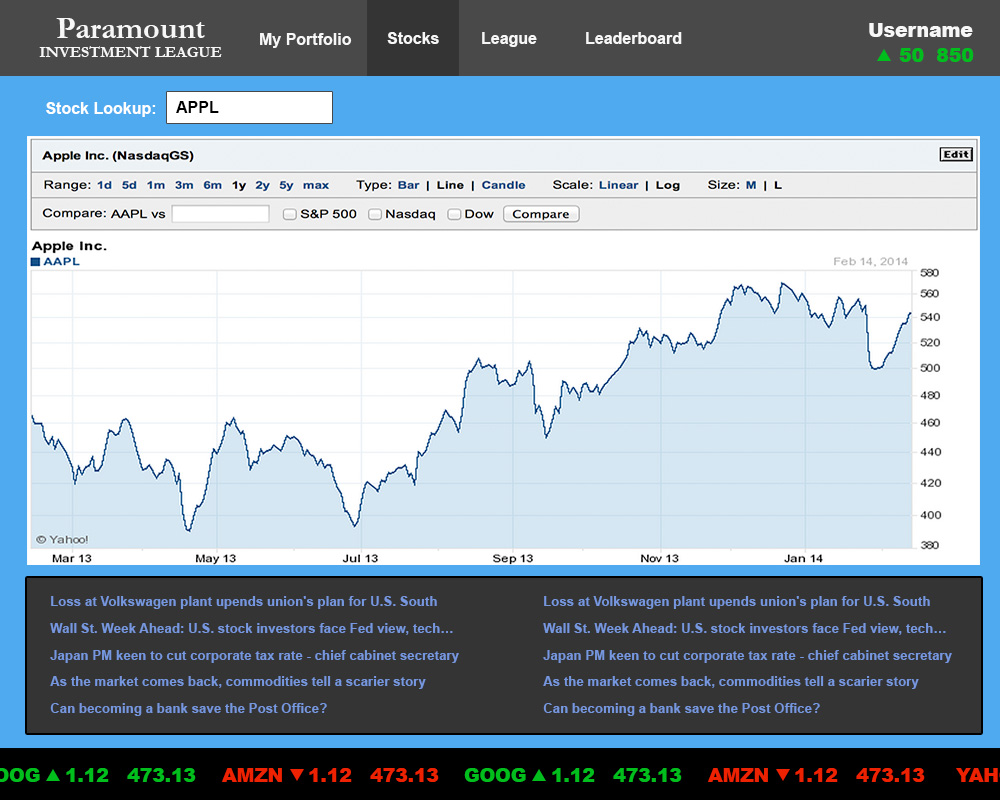
\includegraphics[width=5.5in]{./img/mock/stocks.jpg}
\caption{The preliminary view for asset anaylsis.}
\end{figure}


% This section contains lots of explanations
% of user effort and ease of access
% See Appendix A for examples to boost grade
\section{User Effort Estimation}

Several of the most common usage scenarios for Paramount Investment Leagues:\\

\begin{center}
\begin{tabular}{| l | l | l |}
\hline
\textbf{Usage Scenario} & \textbf{Clicks} & \textbf{Keystrokes} \\ \hline
Login \& Register & 2-3 & 0-1 \\ \hline
Place an Order & 4-6 & 2-12 \\ \hline
Join a League & 3-4 & 0-50 \\ \hline
Create a new League & 6-7 & 11-100 \\ \hline
Analyze Asset & 2 & 2-5 \\ \hline
View Leaderboard & 2 & 0 \\ \hline
\end{tabular}
\end{center}

\subsection{Login \& Register}

Assume the user has come to the domain and wishes to Login if already registered, or
register if already a user:\\
\begin{itemize}
\item \textbf{Navigation: }
\begin{enumerate}
\item Click on OpenID icon (Google, Facebook, Twitter, etc).
\item Click on your account (optional for multiaccounts).
\item Click on login, or hit enter.
\end{enumerate}
\end{itemize}

\subsection{Place an Order}

Assume the user has already logged in and they wish to place an order:\\

\begin{itemize}
\item \textbf{Navigation: }
\begin{enumerate}
\item Navigate to 'My Portfolio', 0-1 clicks.

\end{enumerate}
\item \textbf{Data Entry: }
\begin{enumerate}
\item Select order type from drop down, 2 clicks
\item Click textbox to enter asset name. 1 click
\item Enter assets name eg: 'G', 'O', 'O', 'G', 1-4 keystrokes
\item Press tab to specify number of shares, 1 keystroke (user could also execute 1 click)
\item Enter the number of shares, 1-7 keystrokes
\item Click execute, 1 click
\end{enumerate}
\end{itemize}

\subsection{Join a League}

Assume that the user wishes to join a league and is logged in:\\

\begin{itemize}
\item \textbf{Navigation: }
\begin{enumerate}
\item Click on League, 1 click
\item Click on Join, 1 click
\end{enumerate}
\item \textbf{Data Entry: }
\begin{enumerate}
\item Click on a League, or enter its name, 1 click or up to 50 keystrokes
\item Click on confirmation dialogue, 1 click
\end{enumerate}
\end{itemize}

\subsection{Create a League}

Assume that the user wishes to create a league and is logged in:\\

\begin{itemize}
\item \textbf{Navigation: }
\begin{enumerate}
\item Click on League, 1 click
\item Click on Create, 1 click
\end{enumerate}
\item \textbf{Data Entry: }
\begin{enumerate}
\item Enter its name, 1-50 keystrokes
\item Select ruleset from dropdown, 2 clicks
\item Fill in parameters, 1-2 clicks and 10-50 keystrokes
\item Click on confirmation dialogue, 1 click
\end{enumerate}
\end{itemize}

\subsection{Analyze an Asset}

Assume that the user is logged in and they want to start an in depth analysis of an asset:\\

\begin{itemize}
\item \textbf{Navigation: }
\begin{enumerate}
\item Click on Stock, 1 click
\end{enumerate}
\item \textbf{Data Entry: }
\begin{enumerate}
\item Click on the textbox for entering an asset name, 1 click
\item Enter an asset name, 1-4 keystrokes
\item Hit enter, 1 keystroke
\end{enumerate}
\end{itemize}


\subsection{View Leaderboard}

Assume that the user has logged in and wants to veiw a leaderboard:\\

\begin{itemize}
\item \textbf{Navigation: }
\begin{enumerate}
\item Click on Leaderboard, 1 click
\item Click on Select Legue/Global, 1 click
\end{enumerate}
\end{itemize}

